This section is concerned with the control structure of the WDN. 
\subsection{Control Structure}
This section documents the structure of the control system for this project as seen in \cref{fig:controlstructure}. The intended control structure assumes that the dynamics of the system can be partitioned in two, the fast dynamics of the inertia of the pipes (assuming the pump dynamics are infinitely fast) and the slow dynamics of the tank level.
\begin{figure}[!htb] 
	
	
	\centering
	\begin{tikzpicture}[auto, node distance=2.5cm,>=latex']
		% ========================== Nodes ============================
		% Nodes in upper vertical line
		\node [input, name=rinput] (rinput) {};
		\node [sum, right of=rinput] (sum1) {};
		\node [block, right of=sum1, node distance = 1.5cm] (LQR) {LQR};
		\node [sum, right of=LQR, node distance =
		1.5cm] (sum2) {};
		\node [block, right of=sum2, node distance = 1.5cm] (PI){PI};
		\node [block, right of=PI, align=center] (Fast){Fast\\Dynamics};
		\node [block, right of=Fast, node distance = 3cm, align=center] (Slow){Slow\\Dynamics};
		\node [output, right of=Slow] (output) {};
		
		% Nodes for inner feedback
		\node [tmp, right of=Fast, node distance = 1.5cm] (tmp0){};
		\node [tmp, below of=tmp0, node distance = 1.5cm] (tmp1){};
		\node [tmp, below of=sum2, node distance = 1.5cm] (tmp2){};
		
		% Nodes for outer feedback
		\node [tmp, right of=Slow, node distance = 1.5cm] (tmp10){};
		\node [tmp, below of=tmp10,node distance = 2.5cm] (tmp11){};
		\node [tmp, below of=sum1, node distance = 2.5cm] (tmp12){};
		
		% Nodes for Disturbance
		\node [tmp, above of=tmp0, node distance = 2.5cm] (tmp20){};
		\node [tmp, above of=tmp0, node distance = 2cm] (tmp21){};
		\node [tmp, above of=Fast, node distance = 2cm] (tmp22){};
		\node [tmp, above of=Slow, node distance = 2cm] (tmp23){};
		
		\draw[thick, dotted] ($(Fast.north west)+(-0.25, 0.25)$) rectangle  ($(Slow.south east)+(0.25, -0.25)$);
		\node[above of =tmp0, node distance =1.1cm](sys_txt) {System};
		
		% ========================== Lines ============================
		
		% Lines in upper vertical part of block diagram
		\draw [->] (rinput) -- node{$p_{ref}$} (sum1);
		\draw [->] (sum1) --node[name=z,anchor=north]{} (LQR);
		\draw [->] (LQR) -- node{$ q_{ref} $}(sum2);
		\draw [->] (sum2) -- (PI);
		\draw [->] (PI) -- node[pos=0.4]{$ \omega_{ref} $}(Fast);
		\draw [->] (Fast) -- node{$d_p$}(Slow);
		\draw [->] (Slow) -- node{$p_{\tau}$}(output);	
		
		% Lines for inner feedback
		\draw [-] (tmp0) -- (tmp1);
		\draw [-] (tmp1) -- (tmp2);
		\draw [->] (tmp2) -- node[pos=0.99]{$ - $}(sum2);
		
		
		% Lines for outer feedback
		\draw [-] (tmp10) -- (tmp11);
		\draw [-] (tmp11) -- (tmp12);
		\draw [->] (tmp12) -- node[pos=0.99]{$ - $}(sum1);
		
		
		% Lines for disturbance
		\draw [-] (tmp20)node[above, align=center]{Consumer \\ Disturbance} -- (tmp21);
		\draw [-] (tmp21) -- (tmp22);
		\draw [-] (tmp21) -- (tmp23);
		\draw [->] (tmp22) -- node[left, pos = 0.5]{OD}(Fast);
		\draw [->] (tmp23) -- node[pos = 0.5]{$ d_c $}(Slow);
		
		
	\end{tikzpicture}
	\caption{Control Structure} \label{fig:controlstructure}
\end{figure}


\subsection{System Linearisation}\label{subsec:Linearisation}

Before the model presented in \cref{eq:NonLinearModelWithTank} is truly useful to us - at least within the scope of the \textit{linear} control strategies considered in this project - we must find a way to turn it into a linear model. The typical approach to this problem is \textit{linearisation}, whereby we exploit the extremely powerful Hartman-Grobman theorem, which we present roughly as outlined in \cite{Perko2001}:


\begin{theorem}\label{theorem:HartmanGrobman}
(\textbf{The Hartman-Grobman Theorem}) Let $E$ be an open subset of $\mathbb{R}^n$ containing the origin, and let $f$ be a continuously differentiable function on $E$:
 
\begin{equation*}
f \in C^1(E)
\end{equation*}

Let $\gamma_t$ be the flow of the nonlinear system $\dot{x} = f(x)$. Assume furthermore that there exists an equilibrium point at the origin: 

\begin{equation*}
f(0) = 0
\end{equation*}

and that this equilibrium point is hyberbolic: 

\begin{equation*}
\forall \lambda \in T(A): \ \text{Re}(\lambda) \neq 0, \quad A = \nabla f  
\end{equation*}

where $T$ is the eigenspace of $A$. Then there exists a homeomorphism $H$ of some open set $U, \ 0 \in U$ onto the open set $V, \ 0 \in V$, such that $\forall x_0 \in U$, there is an open interval $I_0 \subset \mathbb{R}, \ 0 \in I_0$ such that:

\begin{equation*}
	\forall x_0 \in U \wedge \forall t \in I_0: \ H \circ \gamma_t(x_0) = e^{At}H(x_0)
\end{equation*}
\end{theorem}

At first glance, this theorem looks opaquely mathematical and not immediately applicable. However, in practice, \cref{theorem:HartmanGrobman} simply tells us that in the immediate vicinity of some hyperbolic equilibrium point of our nonlinear system, there exists a \textit{linear} system that behaves in a generally identical manner when evolved in time. We note that it is not \textit{necessary} to linearise at a hyperbolic equilibrium, but doing so is favourable when possible as it precludes the presence of a center manifold, whose dynamics may not be captured by linearisation.

Recalling that the first-order Taylor series of a function at a point can be thought of as a  generalisation of its tangent line, it is then possible to identify the linearisation of our system via:

\begin{equation}\label{eq:TaylorSeries}
\dot{x} \approx f(x_0) + \nabla f\bigg\rvert_{x_0} (x-x_0)
\end{equation}

We now revert our attention to the nonlinear model of the WDN. We will make the simplifying assumption that $\Phi \mathcal{J} \Phi^T$ is invertible, which is not generally true, but tends to hold for the type of WDN in question. We also introduce the notation $\mathcal{P}: (\Phi \mathcal{J} \Phi^T)^{-1}$, allowing allows us to rewrite \cref{eq:NonLinearModelWithTank} as:

\begin{equation}\label{eq:NonLinearModelSimplified}
	\begin{split}
		\dot{q}_n &=  -\mathcal{P}\Phi\Big(\lambda(q_n)+\mu(q_n,OD)+\alpha(q_n,\omega)\Big) + \mathcal{P}\Big(\Psi(\bar{h}-\mathbf{1}h_0) + \mathcal{I}(p_{\tau}-\mathbf{1}p_0)\Big) \\
		&= 	-\mathcal{P}\Phi\Big(\lambda(q_n)+\frac{|q_n|q_n}{(K_v\cdot OD)^2}+\alpha(q_n,\omega)\Big) + 	\mathcal{P}\Big(\Psi(\bar{h}-\mathbf{1}h_0) + \mathcal{I}(p_{\tau}-\mathbf{1}p_0)\Big) \\
		& = -\mathcal{P}\Phi\Big(K_\lambda|q_n|q_n+\frac{|q_n|q_n}{(K_v\cdot OD)^2}+a_0\omega^2+a_1\omega q+a_2|q|q\Big) + \mathcal{P}\Big(\Psi(\bar{h}-\mathbf{1}h_0) + \mathcal{I}(p_{\tau}-\mathbf{1}p_0)\Big)
	\end{split}	
\end{equation}

We now make the additional observation that $\Psi(\bar{h}-\mathbf{1}h_0)$ is constant for all time,   $\mathcal{I}(p_{\tau}-\mathbf{1}p_0)$ do not depend on $\{q_n,OD,\omega,p_\tau\}$. This suggests that, when computing the Taylor expansion, this term disappears under the action of the $\nabla$ operator, i.e. that:

\begin{equation}\label{eq:PressureHeightDisappear}
	\begin{split}
		\nabla \dot{q}_n &= \nabla \Big(-\mathcal{P}\Phi\Big(\lambda(q_n)+\mu(q_n,OD)+\alpha(q_n,\omega)\Big) + \mathcal{P}\Big(\Psi(\bar{h}-\mathbf{1}h_0) + \mathcal{I}(p_{\tau}-\mathbf{1}p_0)\Big) \\ 
		&=\nabla \Big(-\mathcal{P}\Phi\Big(\lambda(q_n)+\mu(q_n,OD)+\alpha(q_n,\omega)\Big)\Big) + \nabla \mathcal{P}\Big({I}(p_{\tau}-\mathbf{1}p_0)\Big) \\
		&=\nabla \Big(-\mathcal{P}\Phi\Big(K_\lambda|q_n|q_n+\frac{|q_n|q_n}{(K_v\cdot OD)^2}+a_0\omega^2+a_1\omega q+a_2|q|q\Big)\Big) + \nabla \mathcal{P}\Big({I}(p_{\tau}-\mathbf{1}p_0)\Big)
	\end{split}
\end{equation}

Recognizing furthermore that $\Phi$ and $\mathcal{J}$ are simply linear transformations, the linearity of differentiation then allows us to write a general expression for the Taylor expansion of \cref{eq:NonLinearModelSimplified} as:

\begin{equation}\label{eq:SymbolicLinearisation}
	\begin{split}
		\dot{q}_n &\approx f(x_0) + \frac{\partial f}{\partial q_n}\bigg\rvert_{x_0} \tilde{q}_n + \frac{\partial f}{\partial OD}\bigg\rvert_{x_0} \tilde{OD} + \frac{\partial f}{\partial \omega}\bigg\rvert_{x_0} \tilde{\omega} +  \frac{\partial f}{\partial p_\tau}\bigg\rvert_{x_0} \tilde{p}_\tau
		\\
		&= f(x_0) + \mathcal{P}\Big(-\Phi\Big( \frac{\partial \Omega}{\partial q_n}\bigg\rvert_{x_0} \tilde{q}_n + \frac{\partial \Omega}{\partial OD}\bigg\rvert_{x_0} \tilde{OD} + \frac{\partial \Omega}{\partial \omega}\bigg\rvert_{x_0} \tilde{\omega} \Big) + \mathcal{I} \frac{\partial f}{\partial p_\tau}\bigg\rvert_{x_0} \tilde{p}_\tau \Big)
	\end{split}
\end{equation}

where: 

\begin{align}
	x_0 &= \{q_0,OD_0,\omega_0, p_\tau \} \label{eq:EquilibriumPoint} \\
	\Omega &= K_\lambda|q_n|q_n+\frac{|q_n|q_n}{(K_v\cdot OD)^2}+a_0\omega^2+a_1\omega q_n+a_2|q_n|q_n \label{eq:OmegaFun} \\
	\tilde{q}_n &= q_n - q_0 \label{eq:QTilde} \\
	\tilde{OD} &= OD - OD_0 \label{eq:ODTilde} \\ 
	\tilde{\omega} &= \omega - \omega_0 \label{eq:OmegaTilde} \\
	\tilde{p}_\tau &= p_\tau - p_{\tau_0}
\end{align}

Writing out each of the partial derivatives in \cref{eq:SymbolicLinearisation}, we get:

\begin{equation}\label{eq:PartialTaylorQ}
	\frac{\partial \Omega}{\partial q_n}\bigg\rvert_{x_0} 
	=
	a_1\omega_0 + \Big(|q_0|+ \text{sign}(q_0)q_0\Big)\Bigg(K_\lambda + a_2 + \frac{1}{(K_v OD_0)^2}\Bigg) 
\end{equation}

\begin{equation}\label{eq:PartialTaylorOD}
	\frac{\partial \Omega}{\partial OD}\bigg\rvert_{x_0} 
	=
	-|q_0|q_0 \frac{2}{K_v^2 OD_0^3}
\end{equation}

\begin{equation}\label{eq:PartialTaylorOmega}
	\frac{\partial \Omega}{\partial \omega}\bigg\rvert_{x_0} 
	=
	a_1 q_0 + 2a_0\omega_0
\end{equation}

\begin{equation}\label{eq:PartialTaylorPressure}
		\frac{\partial \Omega}{\partial p_\tau}\bigg\rvert_{x_0} 
	=
	1
\end{equation}

and the complete Taylor expansion becomes:

\begin{equation}\label{eq:SymbolicLinearisationExpanded}
	\begin{split}
			\dot{q}_n \approx f(x_0) &-\mathcal{P}\Phi\Bigg(a_1\omega_0 + \Big(|q_0|+\text{sign}(q_0)q_0\Big)\Bigg(K_\lambda + a_2 + \frac{1}{(K_v OD_0)^2}\Bigg) \tilde{q}_n \Bigg)  \\
			&- \mathcal{P}\Phi\Bigg(\Big(-|q_0|q_0 \frac{2}{K_v^2 OD_0^3}\Big) \tilde{OD}\Bigg) \\
			&-  \mathcal{P}\Phi\Bigg(\Big(a_1 q_0 + 2a_0\omega_0\Big) \tilde{\omega}\Bigg) \\
			&+ \mathcal{P} \mathcal{I} \tilde{p}_\tau
	\end{split}
\end{equation}

We will now make three additional abstractions to simplify \cref{eq:SymbolicLinearisationExpanded}. We first exploit the trivial condition that, when linearizing at an equilibrium point, $f(x_0) \equiv 0$. We then consider the fact that, in practice, $OD$ and $p_\tau$ vary very slowly compared to $q_n$ and $\omega$. It is therefore a reasonable assumption that at steady state for the latter variables, the error introduced by neglecting $\frac{\partial\Omega}{\partial OD}$ is:

\begin{equation}\label{eq:IgnoreODError}
	\mathcal{P}\Phi\Big(|\tilde{q}_{ss}|\tilde{q}_{ss}\frac{2}{K_v^2 OD_0^3} \tilde{OD}\Big)
\end{equation}

which, under the assumption that $q_n$ changes much faster than $OD$, is a constant offset and therefore removable by integral action. Analogously, the error induced by ignoring $\frac{\partial\Omega}{\partial p_\tau}$ is: 

\begin{equation}\label{eq:IgnorePressureError}
	\mathcal{P}\mathcal{I}\tilde{p}_\tau
\end{equation}

which is likewise a constant term that may be removed by integral action. Thus, we can restate a greatly simplified form of \cref{eq:SymbolicLinearisationExpanded} as

\begin{equation}\label{eq:SymbolicLinearisationSimplified}
	\dot{q}_n \approx -\mathcal{P}\Phi\Bigg(a_1\omega_0 + \Big(|q_0|+\text{sign}(q_0)q_0\Big)\Bigg(K_\lambda + a_2 + \frac{1}{(K_v OD_0)^2}\Bigg) \tilde{q}_n \Bigg) -  \mathcal{P}\Phi\Bigg(\Big(a_1 q_0 + 2a_0\omega_0\Big) \tilde{\omega}\Bigg)
\end{equation}

\clearpage

\subsection{Linearised model} \label{sec:LinearisedModel}
In the following section state space models are presented both for the fast and the slow system, that is the pump flow and the tank pressure dynamics respectively. 

\subsubsection{State space model - pump dynamics}
Before linearizing the system model, presented in \cref{eq:NonLinearModelWithTank}, we need to identify the equilibrium points. This is done by evaluating the before mentioned model, at fixed $ \omega $ and $ OD $, with dynamic states set to zero. We choose pump speeds as an average of those used in \cref{ap:PumpCoef}, which is $ 66\% $ for each pump. We set OD to $ 0.5 $ for each valve. This yields the following equilibrium point:

	\begin{equation}
	q_C^* = \kbordermatrix{
		\\
		q_3 & 0.1992 \\ 
		q_7 & 0.0231\\
	}
\end{equation}
	\begin{equation}
	\bar{q}_f^* = \kbordermatrix{
		\\
		d_1 & 0.3752 \\ 
		d_5 & -0.2913\\
		q_9 & -0.2876\\
	}
	\end{equation}

\begin{equation}
	d_t^* = 0
\end{equation}


The linearised model of the system can be expressed on the standard state space form given in \cref{eq:StateSpace} by applying the equilibrium to \cref{eq:SymbolicLinearisationSimplified}
\begin{equation}\label{eq:StateSpace}
	\begin{split}
	\dot{x} = Ax + Bu \\
	y = Cx
	\end{split}
\end{equation}

\begin{equation}
	A = \begin{bmatrix}
		-0.3236 & -0.0406 & -0.1577 & 10.0671 & -0.7623 & 0.0000\\
		-0.1429 & -0.3189 & 0.2176 & -1.3489 & -6.0984  & 0\\
		-0.0275 & 0.0687 & -0.3968 & 7.1758 & 1.5246 & 0\\
		0.1089 & 0.0687 & 0.0196 & -20.2792 & 1.5246 & -0.0000\\
		-0.0551 & -0.0443 & -0.0272 & 1.4425 & -15.3466 &   -0.0999\\
		0.1486 & 0.0817 & -0.2877 & 11.1436 & 8.2419 & -0.4174\\
	\end{bmatrix}
\end{equation}

\begin{equation}
	B = \begin{bmatrix}
		0.0982 & 0.0000\\
		0.0078 & 0 \\
		0.1147 & 0 \\
		-0.0408 & 0 \\
		-0.0087 & -0.0193\\
		-0.0651 & -0.0715
	\end{bmatrix}
\end{equation}

The output matrix $ C $ can be constructed by the fact that the two outputs are; the flow pump at the non reference pump and the flow to/from the tank. 

\begin{equation}
C =	\begin{bmatrix}
	&0&0&1&0&0&0\\
	&0&0&-1&-1&-1&-1\\	
\end{bmatrix} 
\end{equation}

The inputs to our system will be the pump speeds. 
The outputs will be the measured pressure at the tank node and the flows of the pumps. This yields
\begin{equation}\label{eq:StateSpaceInputsOutputsFast}
	\begin{split}
		u = \begin{bmatrix} \omega_1 \\ \omega_2	\end{bmatrix} \\
		x = \begin{bmatrix} q_c \\ d_f \\ d_{\tau}	\end{bmatrix} \\
		y = \begin{bmatrix} d_1 \\ d_{13} \\ 	\end{bmatrix} \\
	\end{split}
\end{equation}

\subsubsection{State space model - tank pressure dynamics}
The tank pressure dynamics are significantly simpler than the fast dynamics of the system - in fact, the slow tank pressure dynamics of the system are a linear first-order system that, per \cref{eq:TankDynamics}, evolve according to:

\begin{equation}\label{eq:SlowTankDynamics}
	\begin{split}
		\dot{p}_\tau &= - \tau d_\tau \\
		&= \tau \left(d_1 + d_{13} + d_5 + d_9\right)
	\end{split}
\end{equation}

We can discretize this with Euler's method, resulting in:

\begin{equation}\label{eq:TankDynamicsDiscrete}
	\begin{gathered}
			p_\tau(k+1) = p_\tau(k) + \tau \left(d_1(k) + d_{13}(k) + d_5(k) + d_9(k)\right)t_s = T\left(d_1(k) + d_{13}(k) + d_5(k) + d_9(k)\right) \\ 
			T = \tau\cdot t_s 
	\end{gathered}
\end{equation}

which can be converted into the following state-space system:

\begin{equation}\label{eq:TankPressureStateSpace}
	\begin{gathered}
				p_\tau(k+1) = A p_\tau(k) + B_pd_p(k) + B_cd_c(k)
				= A p_\tau(k) + \left(B_p \begin{bmatrix}d_1(k) \\ d_{13}(k)\end{bmatrix} 
				+ B_c\begin{bmatrix}d_5(k) \\ d_9(k)\end{bmatrix}\right) \\      
				A = 1, \ B_p = \begin{bmatrix}T & T \end{bmatrix}, \ B_c = \begin{bmatrix}T & T\end{bmatrix}
	\end{gathered}
\end{equation}

In practice the flows may not all be measurable, in which case they must be estimated with an observer. As \cref{eq:TankPressureStateSpace} is clearly linear, either a simple Luenberger observer or a Kalman filter will do. Additionally, we note the presence of $B_cd_c$, an exogenous input over which we have no control. This will be addressed in \cref{sec:LQR,sec:KalmanFilter}.

\subsection{Influence of pump delay}
The pumps of the WDN system introduces a delay of approximately 4 seconds. According to \cite{Skogestad2005} (pp. 182-183), 
a time delay $\theta$ limits the possible bandwidth of a system to be 

\begin{equation}\label{eq:BWdelay}
	\omega_c < \frac{1}{\theta}
\end{equation}

This naturally sets a limitation as to how fast the inner loop of the control structure can be. As the inner loop sets a limitation of how fast the outer loop can be, i.e. 5-10 timer slower than the inner loop. This is a nessesary limitation, since the inner loop needs to be sufficiently fast for it to be used to linearize the outer loop. 

\subsection{Design of pump controllers}
This section will cover design of pump controllers, which corresponds to control of the fast dynamics of the system. It is also considered the inner loop. 
\subsubsection{Decentralised control}
Based on the obtained linearised model, controllers for the pumps are being introduced. Its desired to obtain decentralised control as this mitigates network faults and decrease delays in the system. Decentralised control can be obtained in a MIMO system if the plant is close to diagonal, meaning that the system can be considered a collection of independent sub-systems \cite{Skogestad2005} p. 91. 
In order to validate whether decentralised control can be obtained, the interactions in the off diagonals of the systems are investigated with magnitude plots. For this analysis the tank is assumed to have a constant pressure. This is part of the seperation of the inner and outer loop, where the outer loop is assumed to be sufficienly slow, so it can be ignored in analysis of the inner loop. The magnitude plots can be seen in \cref{fig:PumpMagPlot}. They show the gain from a input frequency $\omega$ on each of the pumps to the output flows of the pumps.

\begin{figure}[h!]
	\centering
		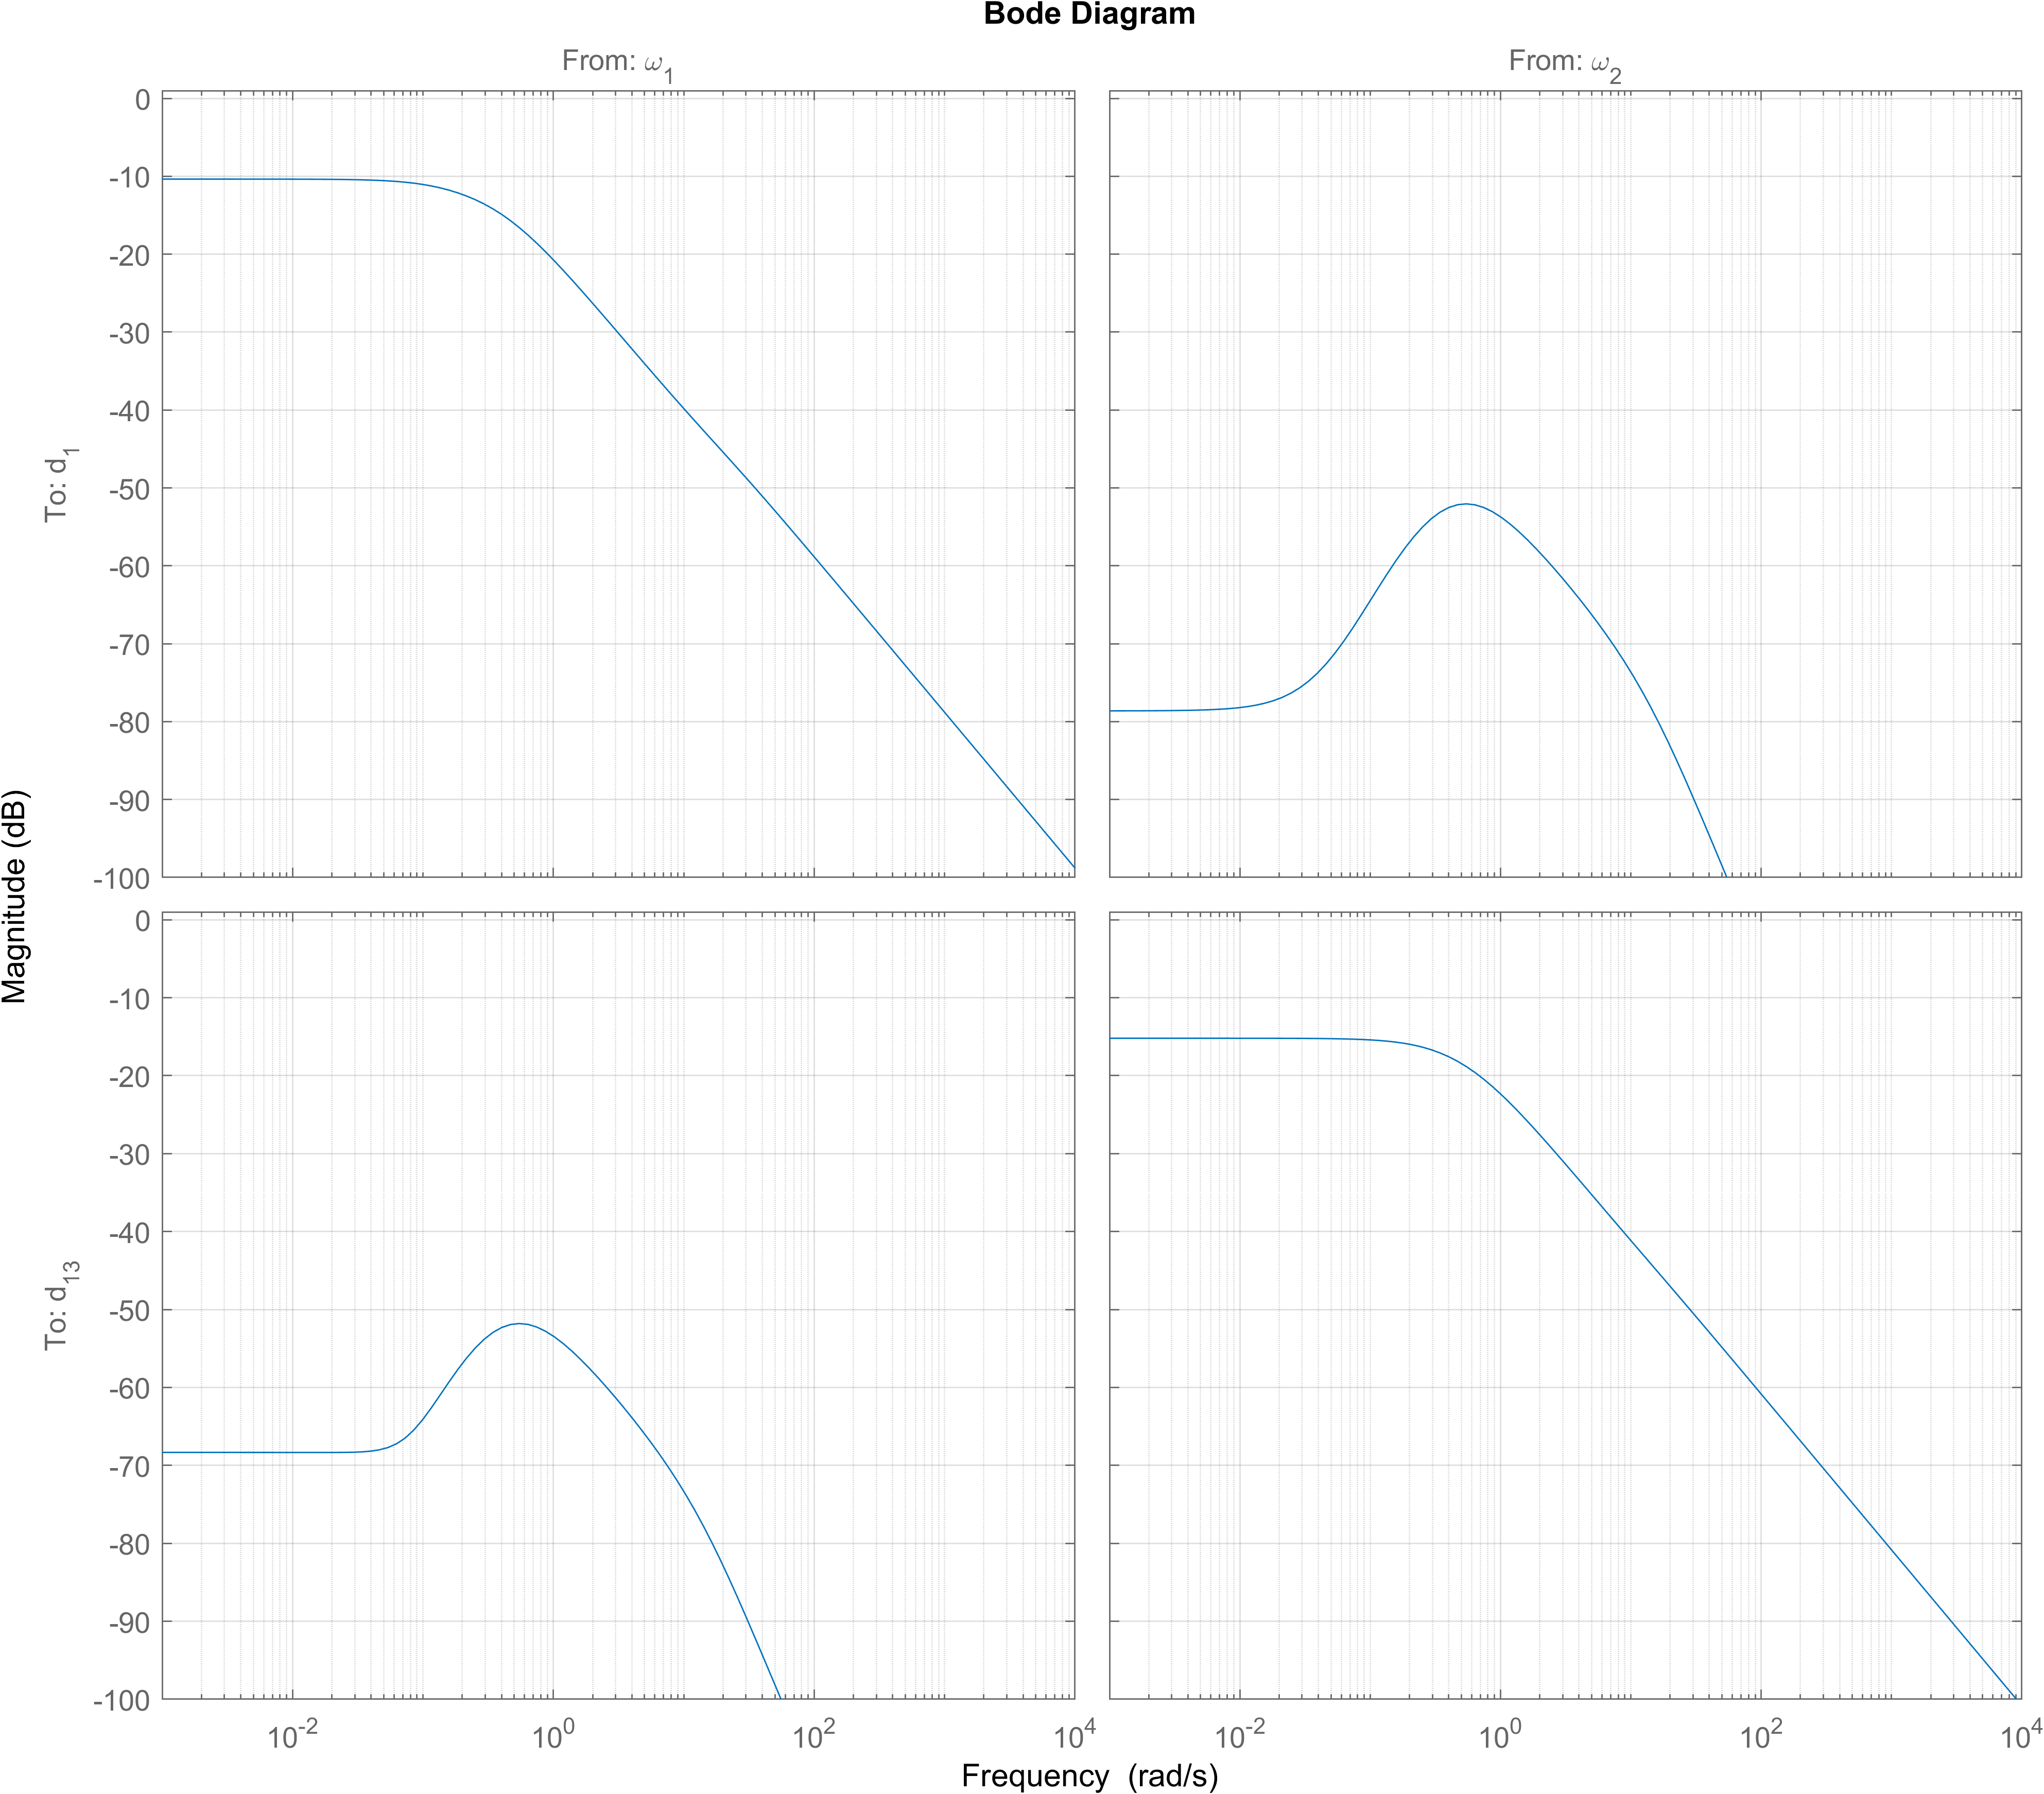
\includegraphics[width=0.8\textwidth]{Pictures/PumpMagPlot.png}
		
		\caption{Magnitude Plot from inputs to outputs}
	\label{fig:PumpMagPlot}
\end{figure}

As seen in \cref{fig:PumpMagPlot}, the gain from $\omega_1$ to $d_{13}$ is for all frequencies less than -50 dB, compared to -10 dB from $\omega_1$ to $d_1$. \\
Likewise is the gain from $\omega_2$ to $d_1$ for all frequencies less than -50 dB, compared to -15 dB from $\omega_2$ to $d_{13}$.\\
In both cases, the coupling is at least -35 dB corresponding to less than a factor of 1/50. Thus the system will be assumed to have no interaction/coupling, which allows for design of controllers independently of the interactions, and solely from the diagonal transfer functions in the transfer matrix.

\subsubsection{Similarities within the diagonal systems and simplification}
The diagonal transfer functions are considered to be identical, based on the poles and zeros of the two diagonal transfer functions seen in \cref{eq:PumpDiagonalPolesZeros}: 

\begin{equation}\label{eq:PumpDiagonalPolesZeros}
	\begin{gathered}
		z_{11} = \begin{bmatrix}-18.9173&  -13.9942&   -0.5571&   -0.3357&   -0.1944 \end{bmatrix} \\
		z_{22} = \begin{bmatrix}-20.7216&  -14.1600&   -0.4079&   -0.3639&   -0.1597 \end{bmatrix} \\
		p_{11} = p_{22} = \begin{bmatrix} 20.7703&  -14.8635&   -0.5624&   -0.3930&   -0.3337&   -0.1597 \end{bmatrix} \\
	\end{gathered}
\end{equation}

Considering the two systems identical enables the design of only one controller for both the subsystems.\\
Realising that many of the poles more or less cancels out with the zeros can simplify the model very much for the root locus design, yielding poles and zeros \cref{eq:SimplifiedPolesZeros}:

 \begin{equation}\label{eq:SimplifiedPolesZeros}
 	\begin{gathered}
 		z = \begin{bmatrix}  -0.1944 \end{bmatrix} \\
 		p = \begin{bmatrix}  -0.3930&  -0.1597 \end{bmatrix} \\
 	\end{gathered}
 \end{equation}

\subsubsection{Modelling of time delay}
The timedelay of the pumps can be modelled with a pade approximation, using Matlab. The order of the approximation is not unimportant. The higher the order, the closer to a true time delay the result will be. It comes however at the cost of clarity, as a nth-order approximation places \textit{n} LHP poles and \textit{n} RHP zeroes, to simulate the delay. This is shown in \cref{fig:PadeApprox}.
\begin{figure}[h!]
	\centering
	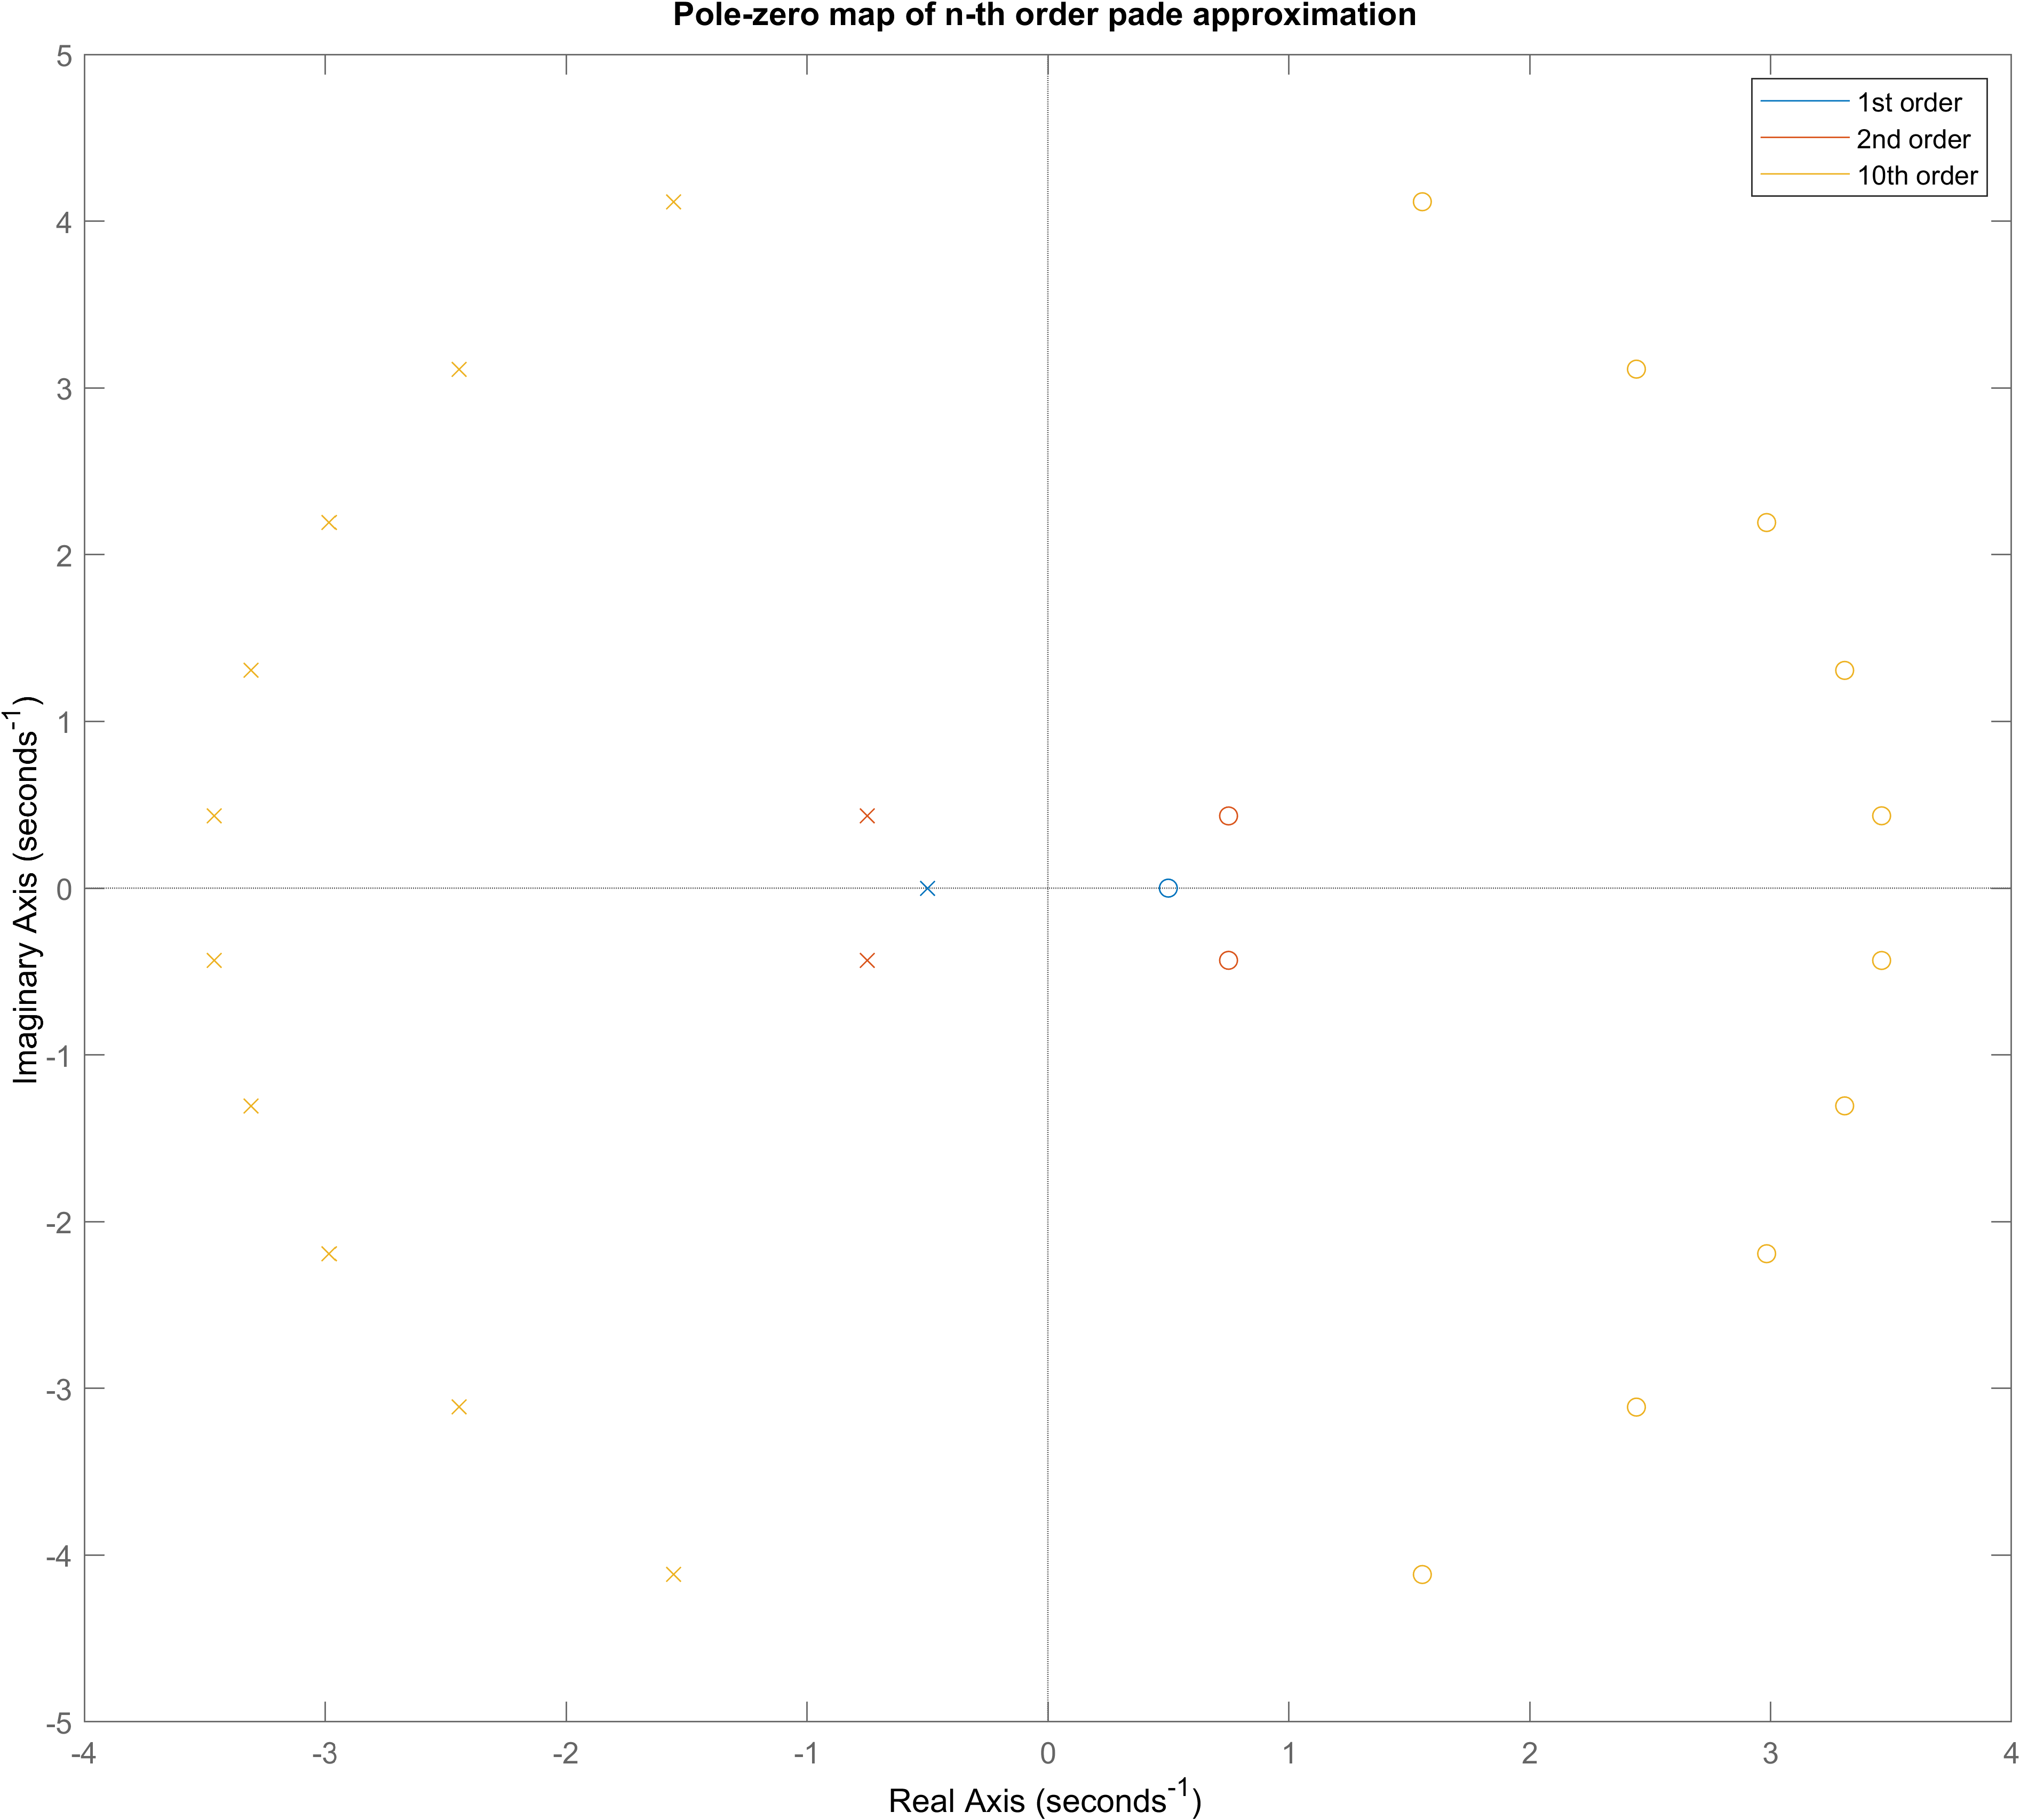
\includegraphics[width=0.8\textwidth]{Pictures/PadeApprox.png}
	\caption{Pole-zero map of various order pade approximations of a 4 second delay}
	\label{fig:PadeApprox}
\end{figure}

An investigation has been performed to show the error in closed loop pole locations introduced by using a low order approximation. \cref{fig:CLPoles} and \cref{fig:CLPolesZoom} shows the closed loop pole locations when using a 1st, 2nd and 10th order pade approximation. The plots show a noticable difference from 1st to 2nd order, but no significance above that.

\begin{figure}[h!]
	\centering
	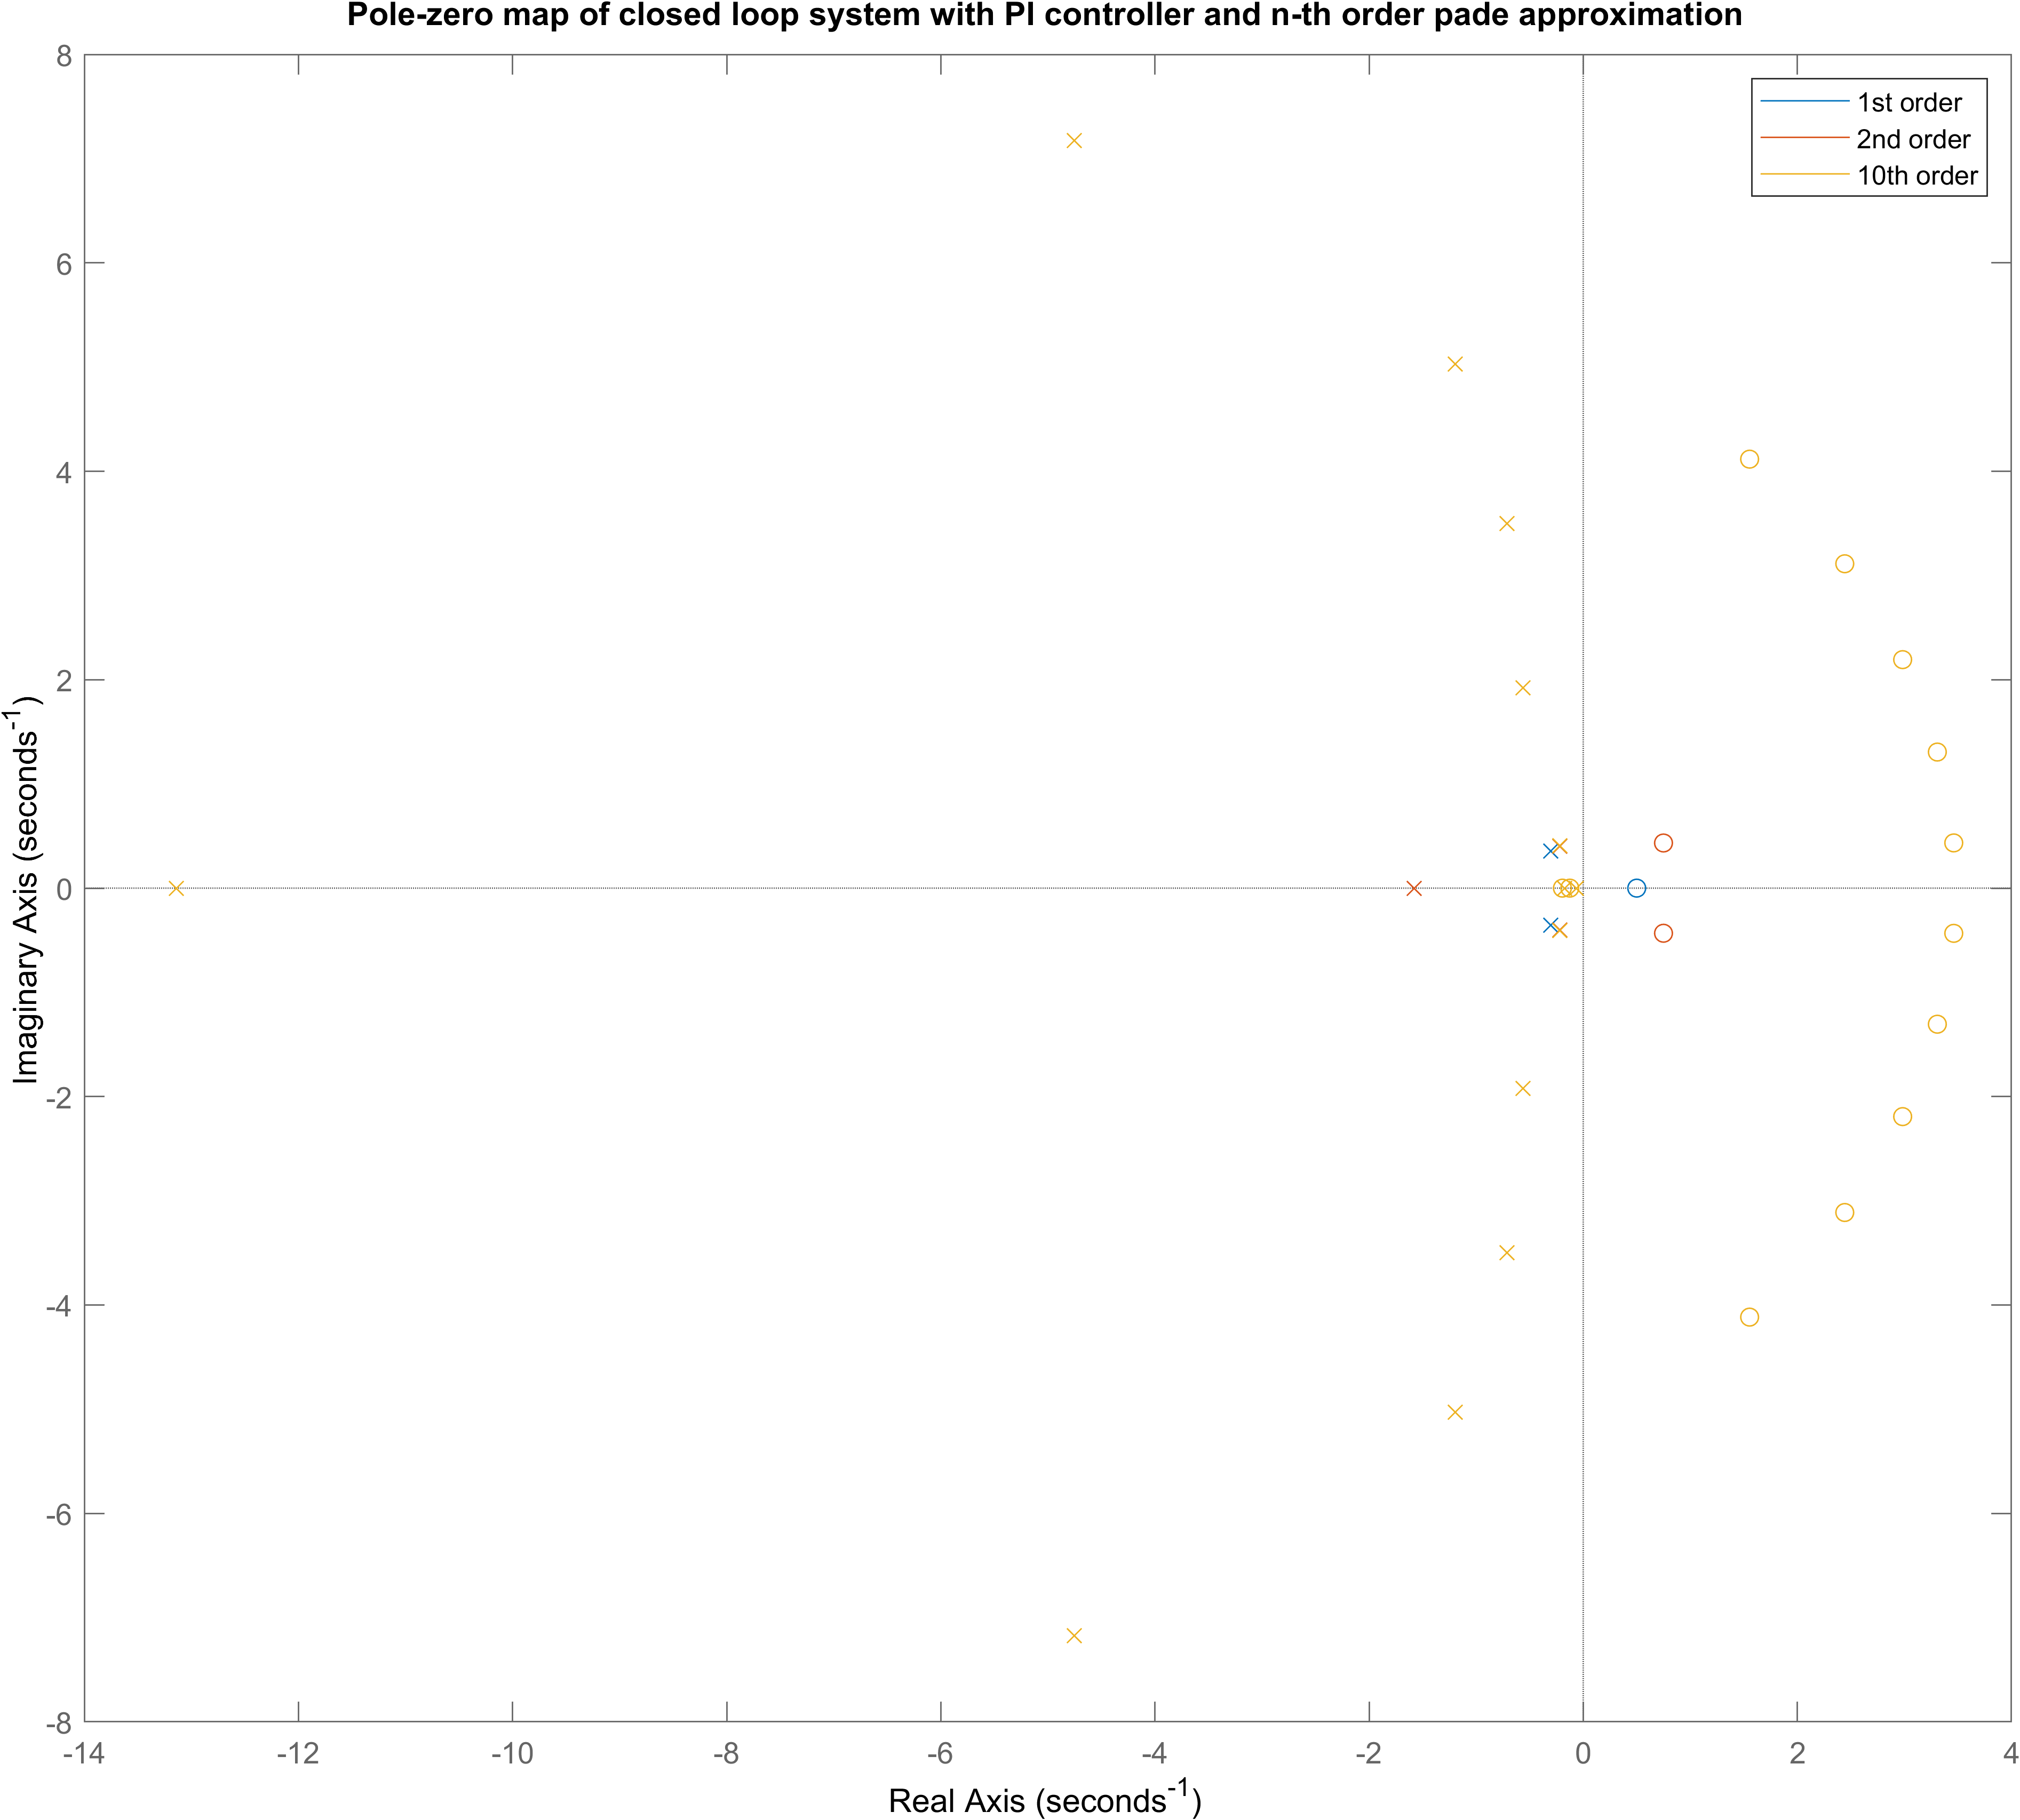
\includegraphics[width=0.8\textwidth]{Pictures/PZmap_CL.png}
	\caption{Pole-zero map of closed loop pole locations with various order pade approximations of a 4 second delay}
	\label{fig:CLPoles}
\end{figure}
\begin{figure}[h!]
	\centering
	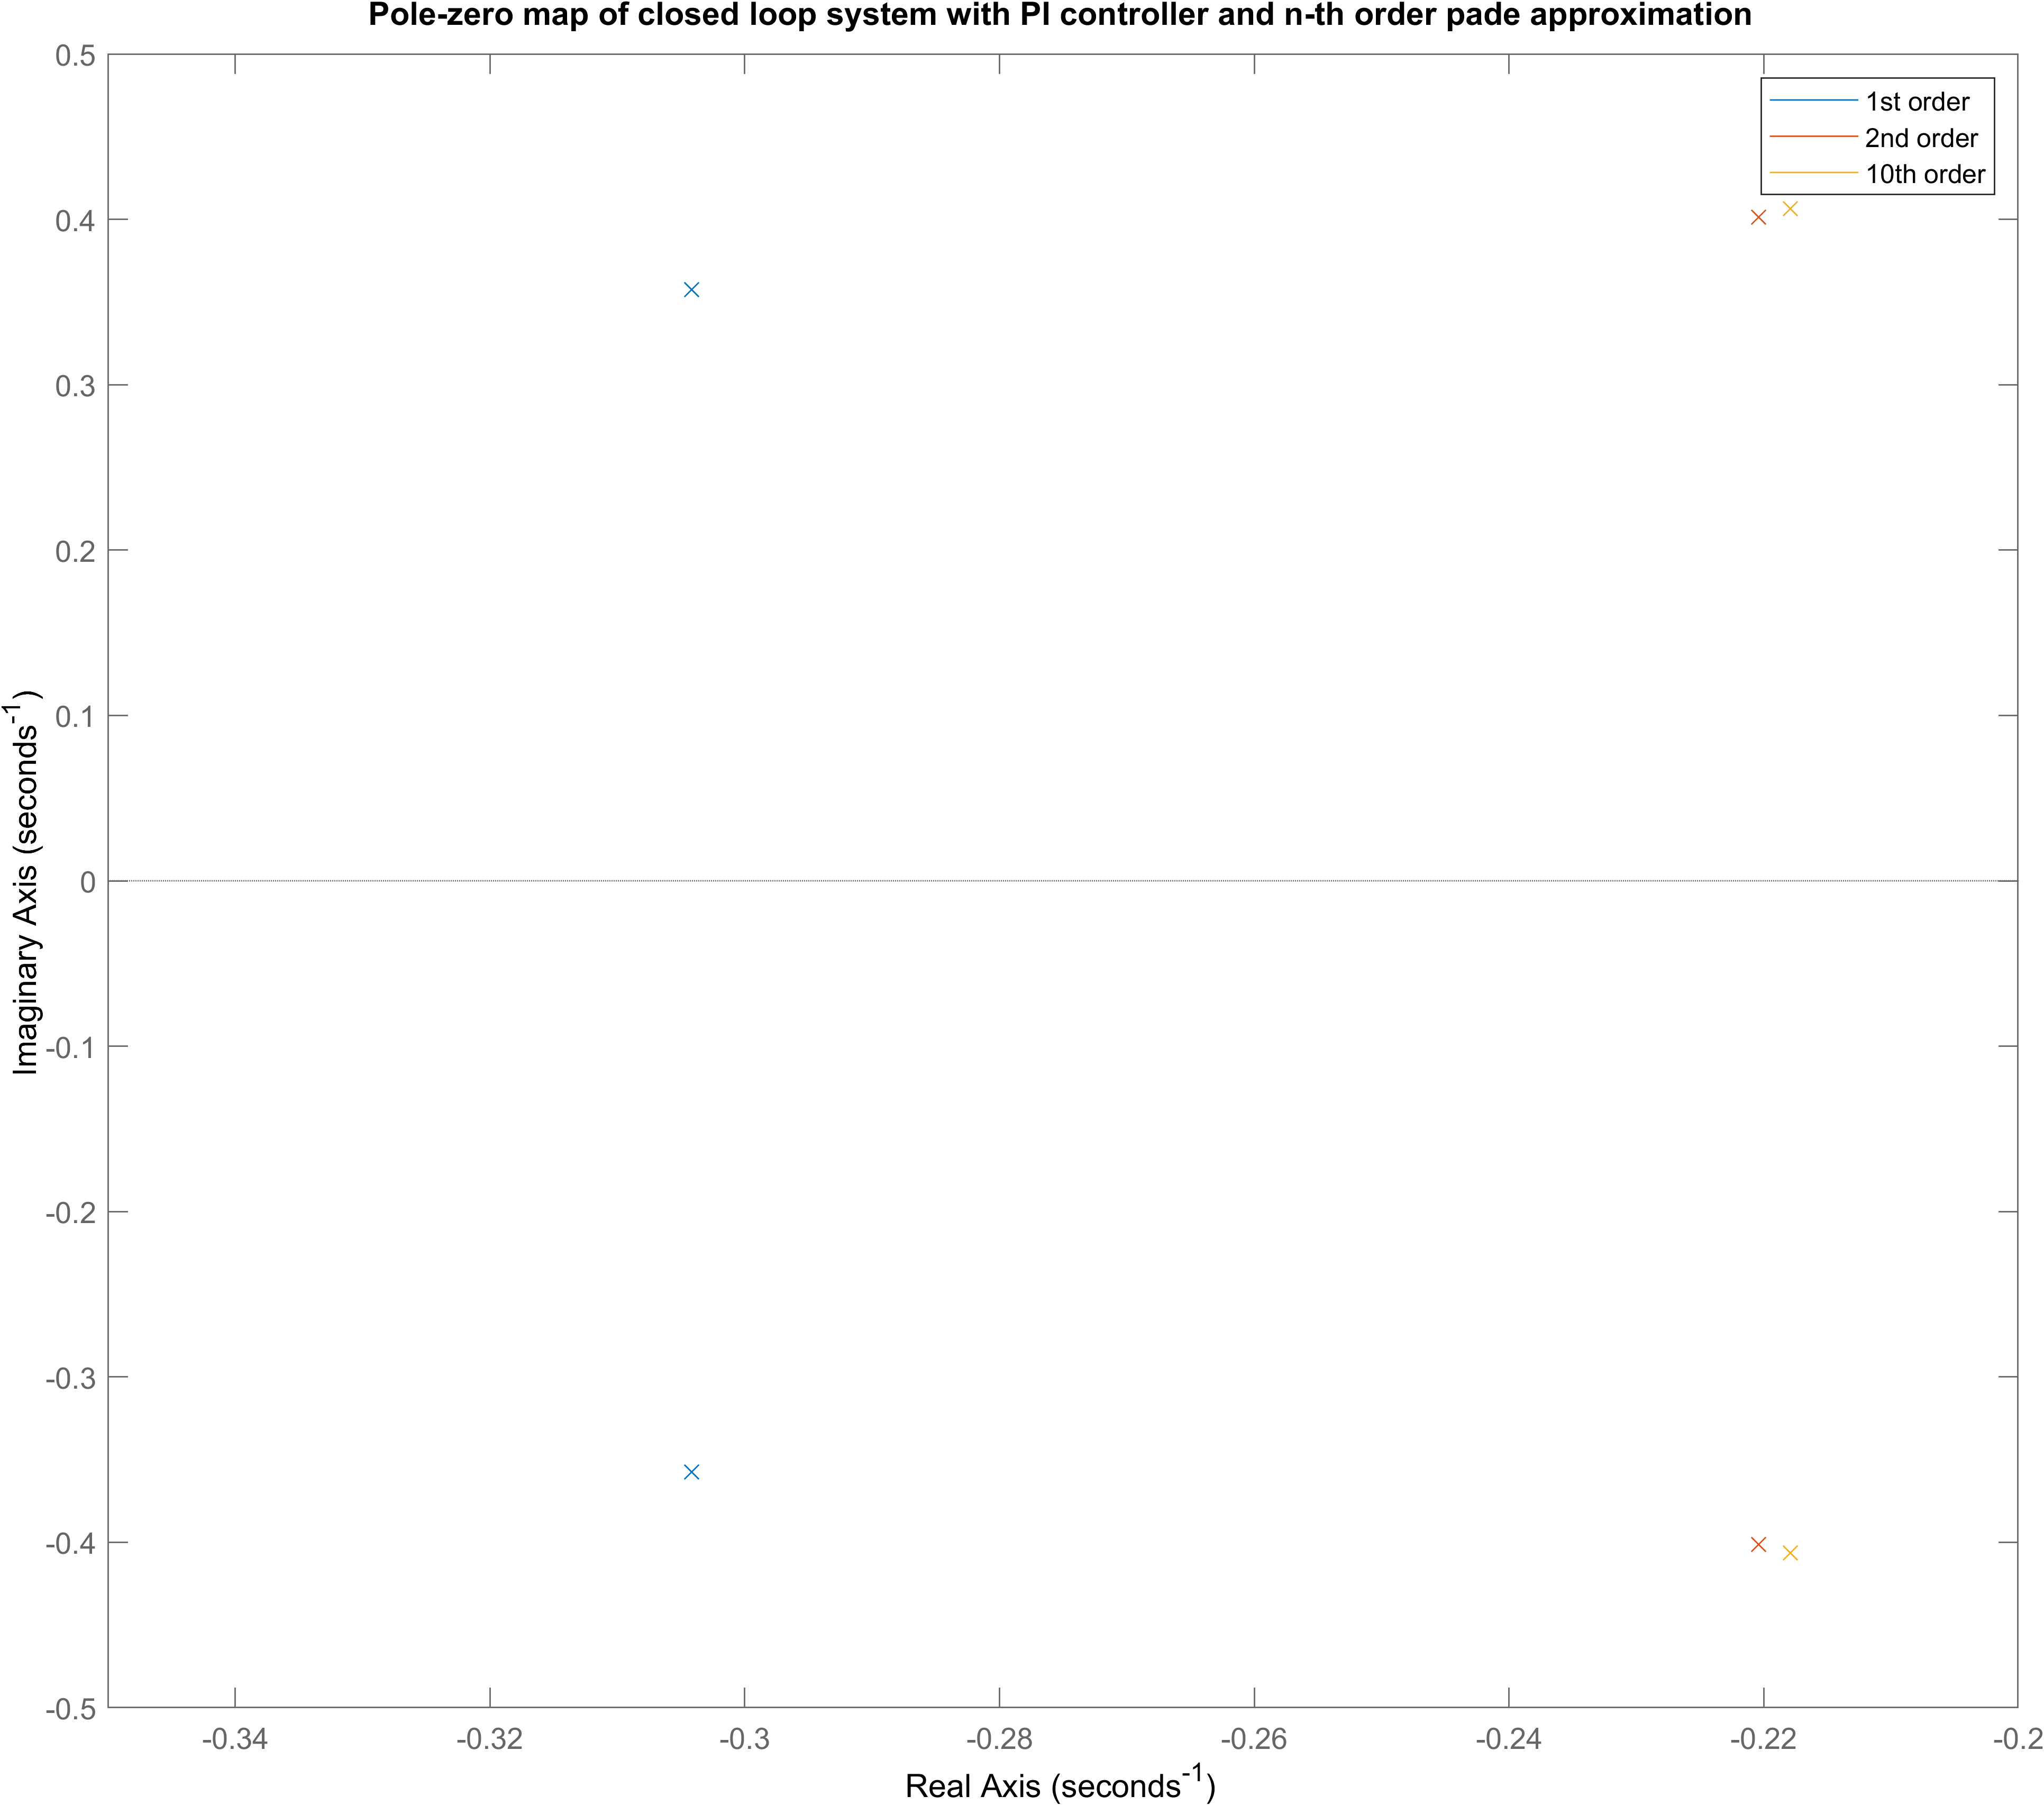
\includegraphics[width=0.8\textwidth]{Pictures/PZmap_CL_zoom.png}
	\caption{Pole-zero map of closed loop pole locations with various order pade approximations of a 4 second delay. Zoomed in on the dominant complex conjugate pole pair.}
	\label{fig:CLPolesZoom}
\end{figure}
When considering both convenience of use and modelling error the optimal approximation order was chosen to be 2.


\subsubsection{Requirements for control performance}
Before starting the actual root locus design of the controller, the desired performance of the controlled system needs to be defined. \\
The first priority of the controlled system is for it to be stable. This is achived by ensuring that the closed loop poles of the system are placed in the left half plane on the s-plane. Simultaniously the inner loop of the system should be at least 5 times faster than the slow outer system [we have to come up with a reasonable estimate of this]. The desired BW of the inner loop is chosen to be 0.1 rad/s. This in turn is another restriction on the closed loop pole locations.

Next, the controlled system should have no steady state error for step inputs. This ensures that the outer controller freely can set and achieve the desired pump flow reference. Lastly the system should have no overshoot and low amount of oscilations in its stepresponse, to indicate a sound phase margin to accommodate model uncertainty.

Since the transfer function of the desired subsystem can be simplified as having two real poles and one zero, and the pade approximation adds two complex poles and zeros, the system can not be described as a second order system. Therefore traditional requirements like damping ratio do not apply in the normal sense. The requirements will thus be simpler, allowing more freedom for the designer to tune the controller based on the actual stepresponse.

The requirements for the controller can be condensed to the following: 
\begin{itemize}
	\item No poles must be in the right half plane.
	\item An open loop pole must be placed in the origin.
	\item The closed loop system must have a bandwidth of approximately 0.1 rad/s.
	\item The closed loop system must have a time constant of approximately $\frac{1}{bw} = \frac{1}{0.1} = 10s$.
\end{itemize}



\subsubsection{Choice of controller type}
A PI controller is considered to be a sufficient solution for the requirements put forth. The integral action will take care of the steady state error, and the gain and zero location can be chosen based on the design criteria.

\subsubsection{Root locus design}
Since the controller is to be used locally for one pump, the root locus is drawn for the transfer function that takes the rotational speed of pump 1 as input and the resulting flow of pump 1 as output. The transfer function is in reduced form, where close pole-zero pairs have been cancelled out. The 2nd order pade approximation of a 4 second time delay is included.


The controller design is then performed in four steps:
\begin{enumerate}
	\item Place one pole at the origin.
	\item Place one real zero in the left half plane.
	\item Select a gain K that yields optimal closed loop poles.
	\item Evaluate the step response and readjust the zero location and gain value if needed.
\end{enumerate}

While step 1 requires no intuition, step 2 has to be done rather carefully. Placing the zero too close to the origin will slow down the integration drastically. Placing it too far to the left however, creates a loci where the possible closed loop poles are all undesireable.

For step 3, the gain was increased until the bandwidth of 0.1 rad/s was achieved with no oscilations. 

As step 4 implies, the PI controller was designed after some iterations, resulting in the following controller:

 \begin{equation}\label{eq:PITransferFunction}
	G_{PI} = 1.8 \frac{s+0.125}{s}
\end{equation}

With this controller the root locus can be seen on \cref{fig:RootLocus_PadeTwo}. The plot show zeroes as o's, poles as x's and closed loop poles as red dots.
\begin{figure}[h!]
	\centering
	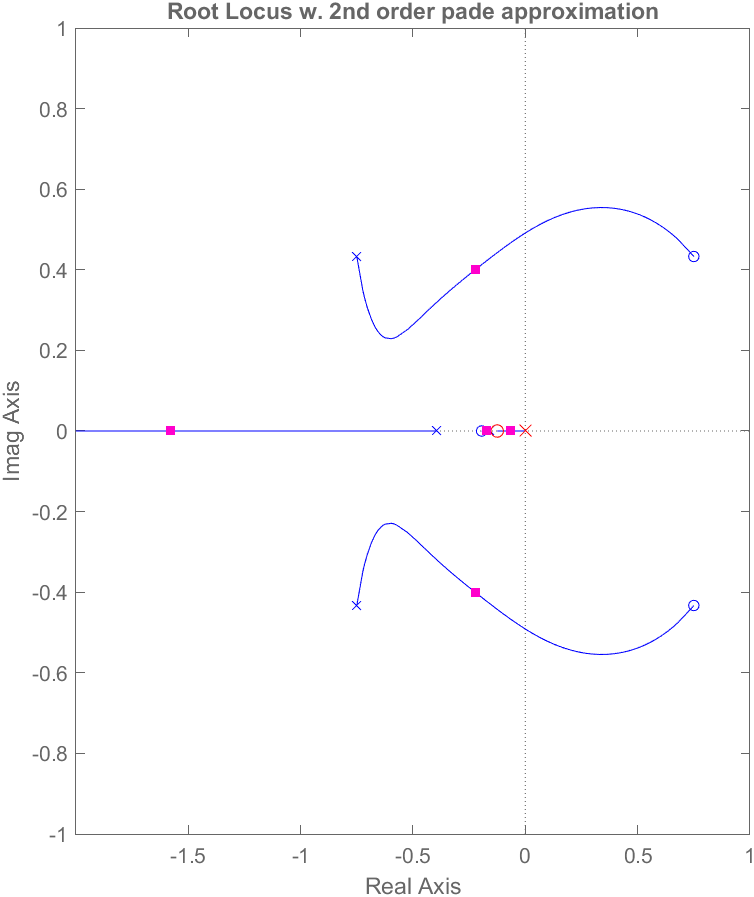
\includegraphics[width=0.8\textwidth]{Pictures/RootLocus_Pade2.png}
	
	\caption{Root locus of delayed pump transfer function with PI controller}
	\label{fig:RootLocus_PadeTwo}
\end{figure}

The resulting closed loop step response is seen on \cref{fig:StepResponse_Pade2}. The step response shows an initial undershoot. This is not a result of the physical system, but rather the pade approximation, which places zeroes in the right half plane. These zeroes cause the step response to undershoot in an attempt to delay the signal. Increasing the order of approximation can reduce this, as shown in \cref{fig:StepResponse_Pade10}. \cref{fig:StepResponse_Pade10} also shows that no significant error in the step response is caused by using a 2nd order approximation rather that 10th order.

\begin{figure}[h!]
	\centering
	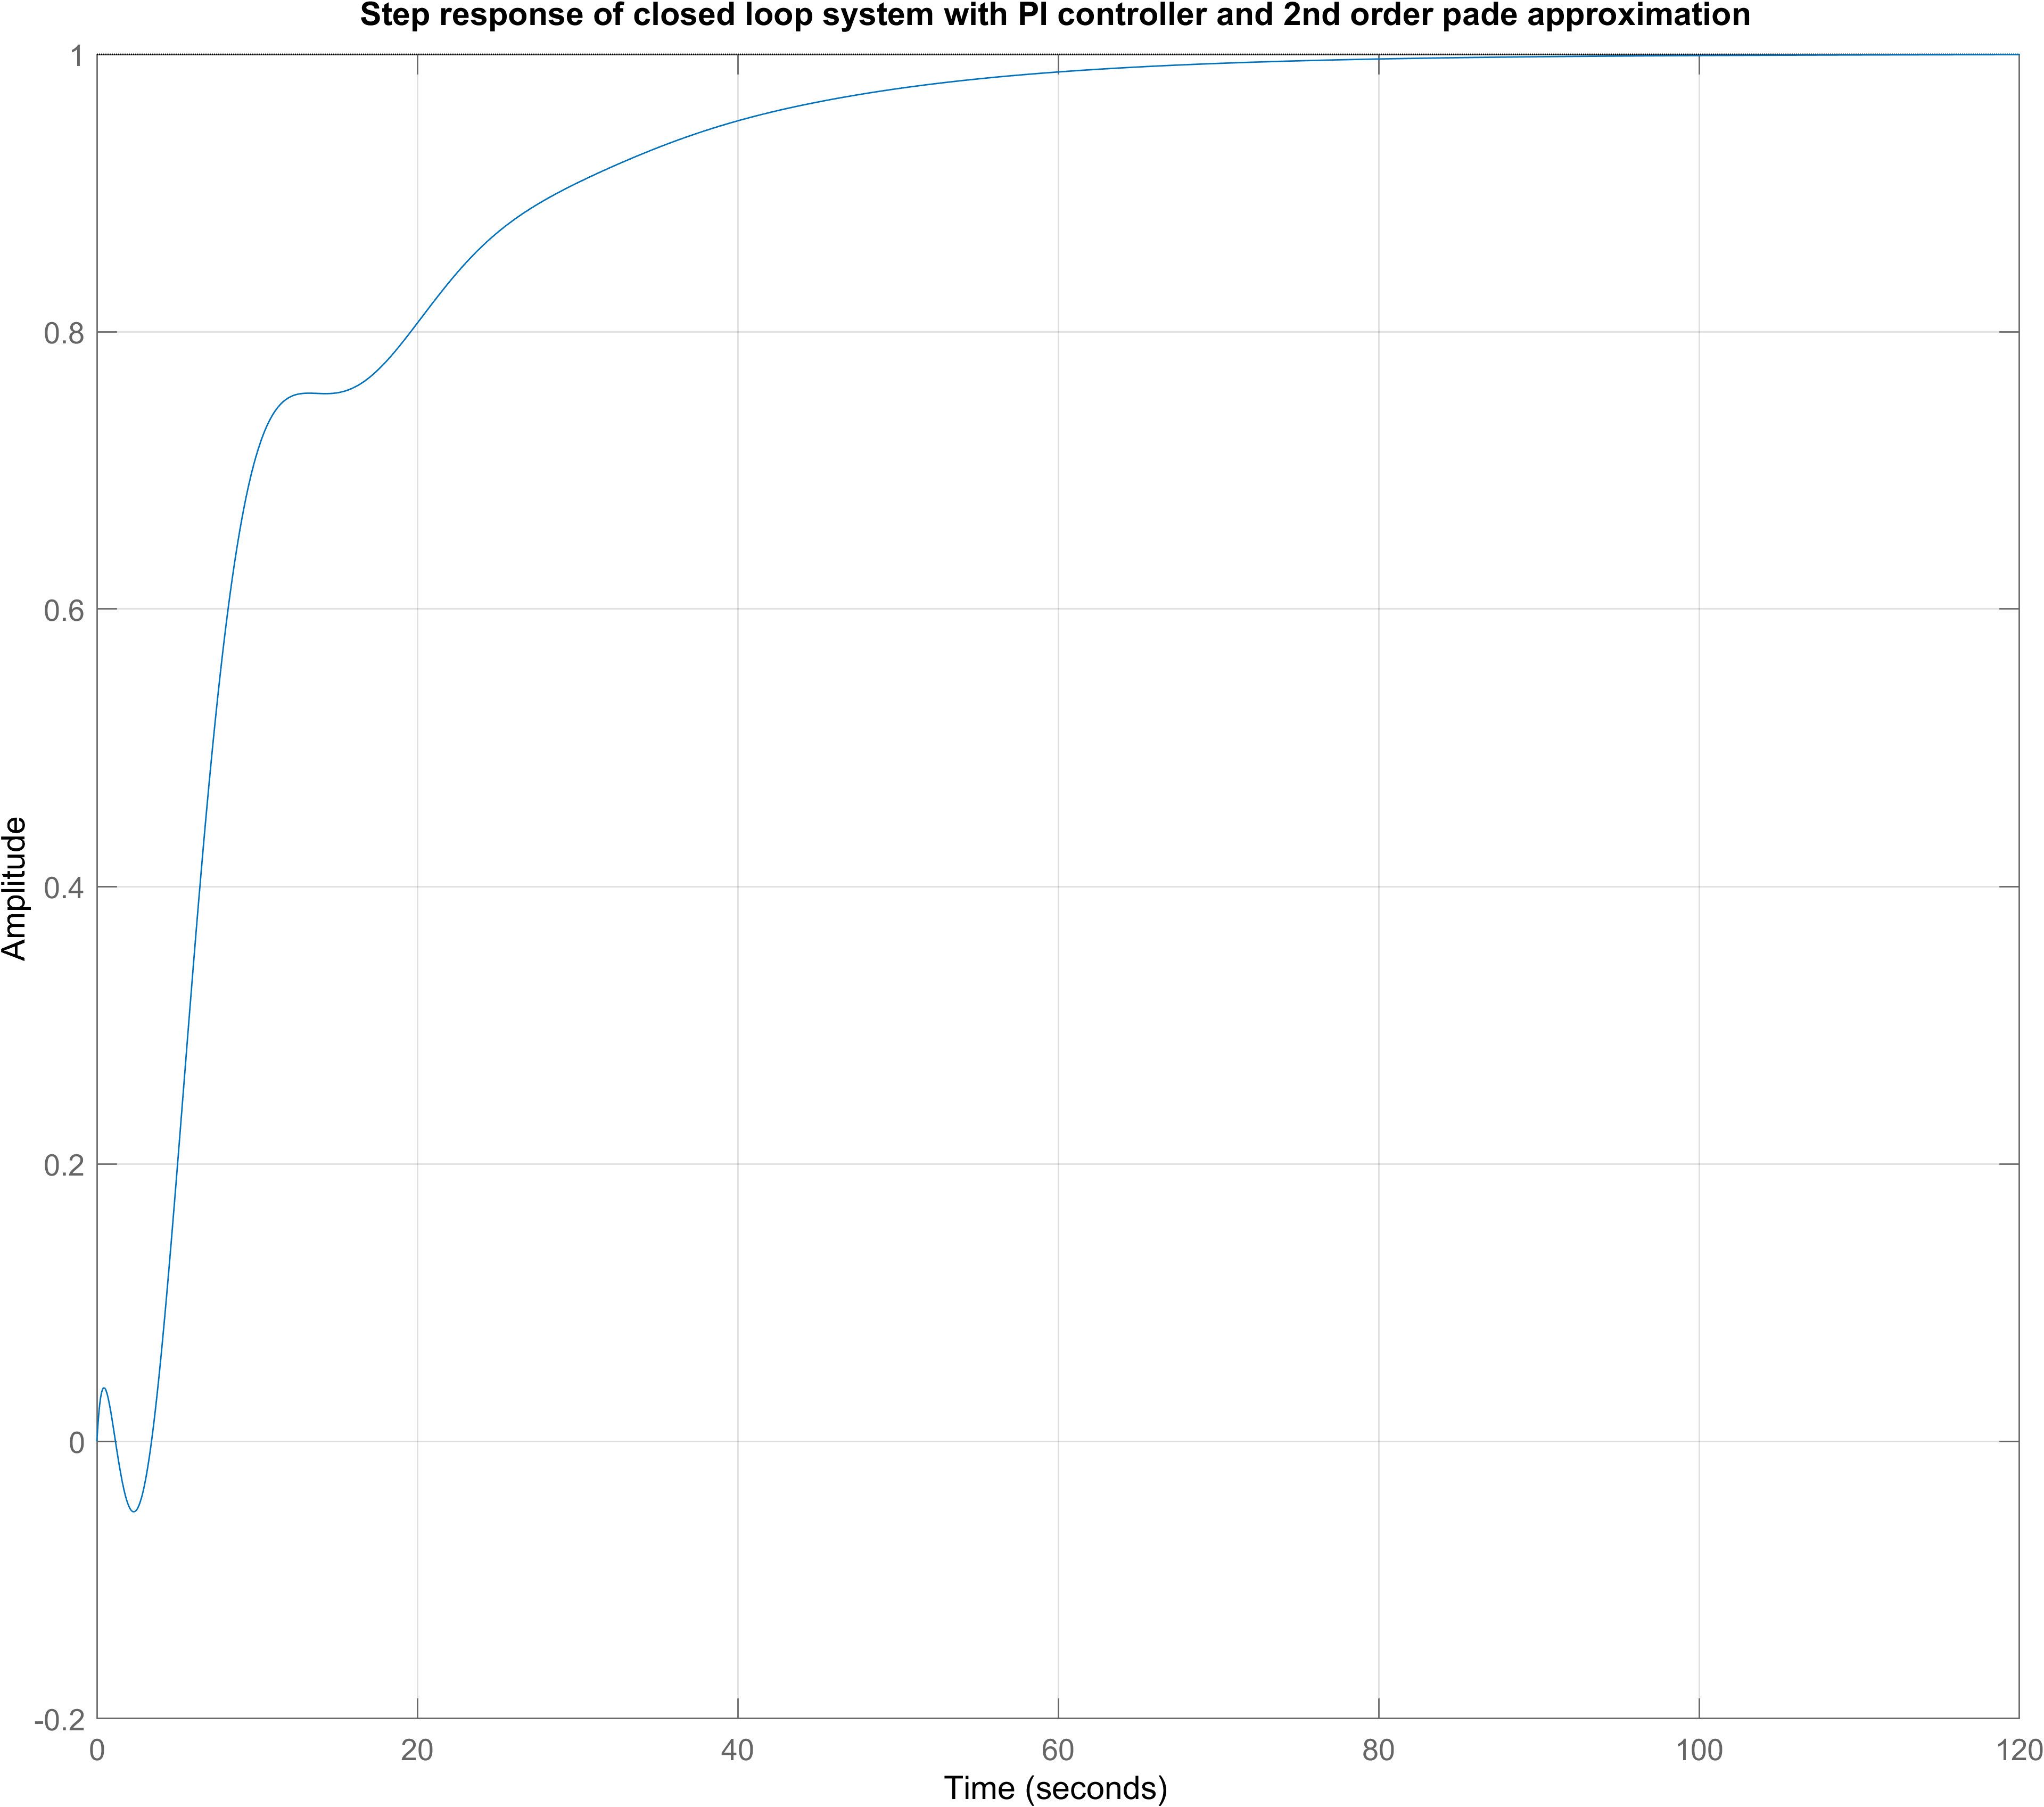
\includegraphics[width=0.8\textwidth]{Pictures/StepResponse_Pade2.png}
	
	\caption{Step response of the closed loop system with a 2nd order pade approximation}
	\label{fig:StepResponse_Pade2}
\end{figure}


\begin{figure}[h!]
	\centering
	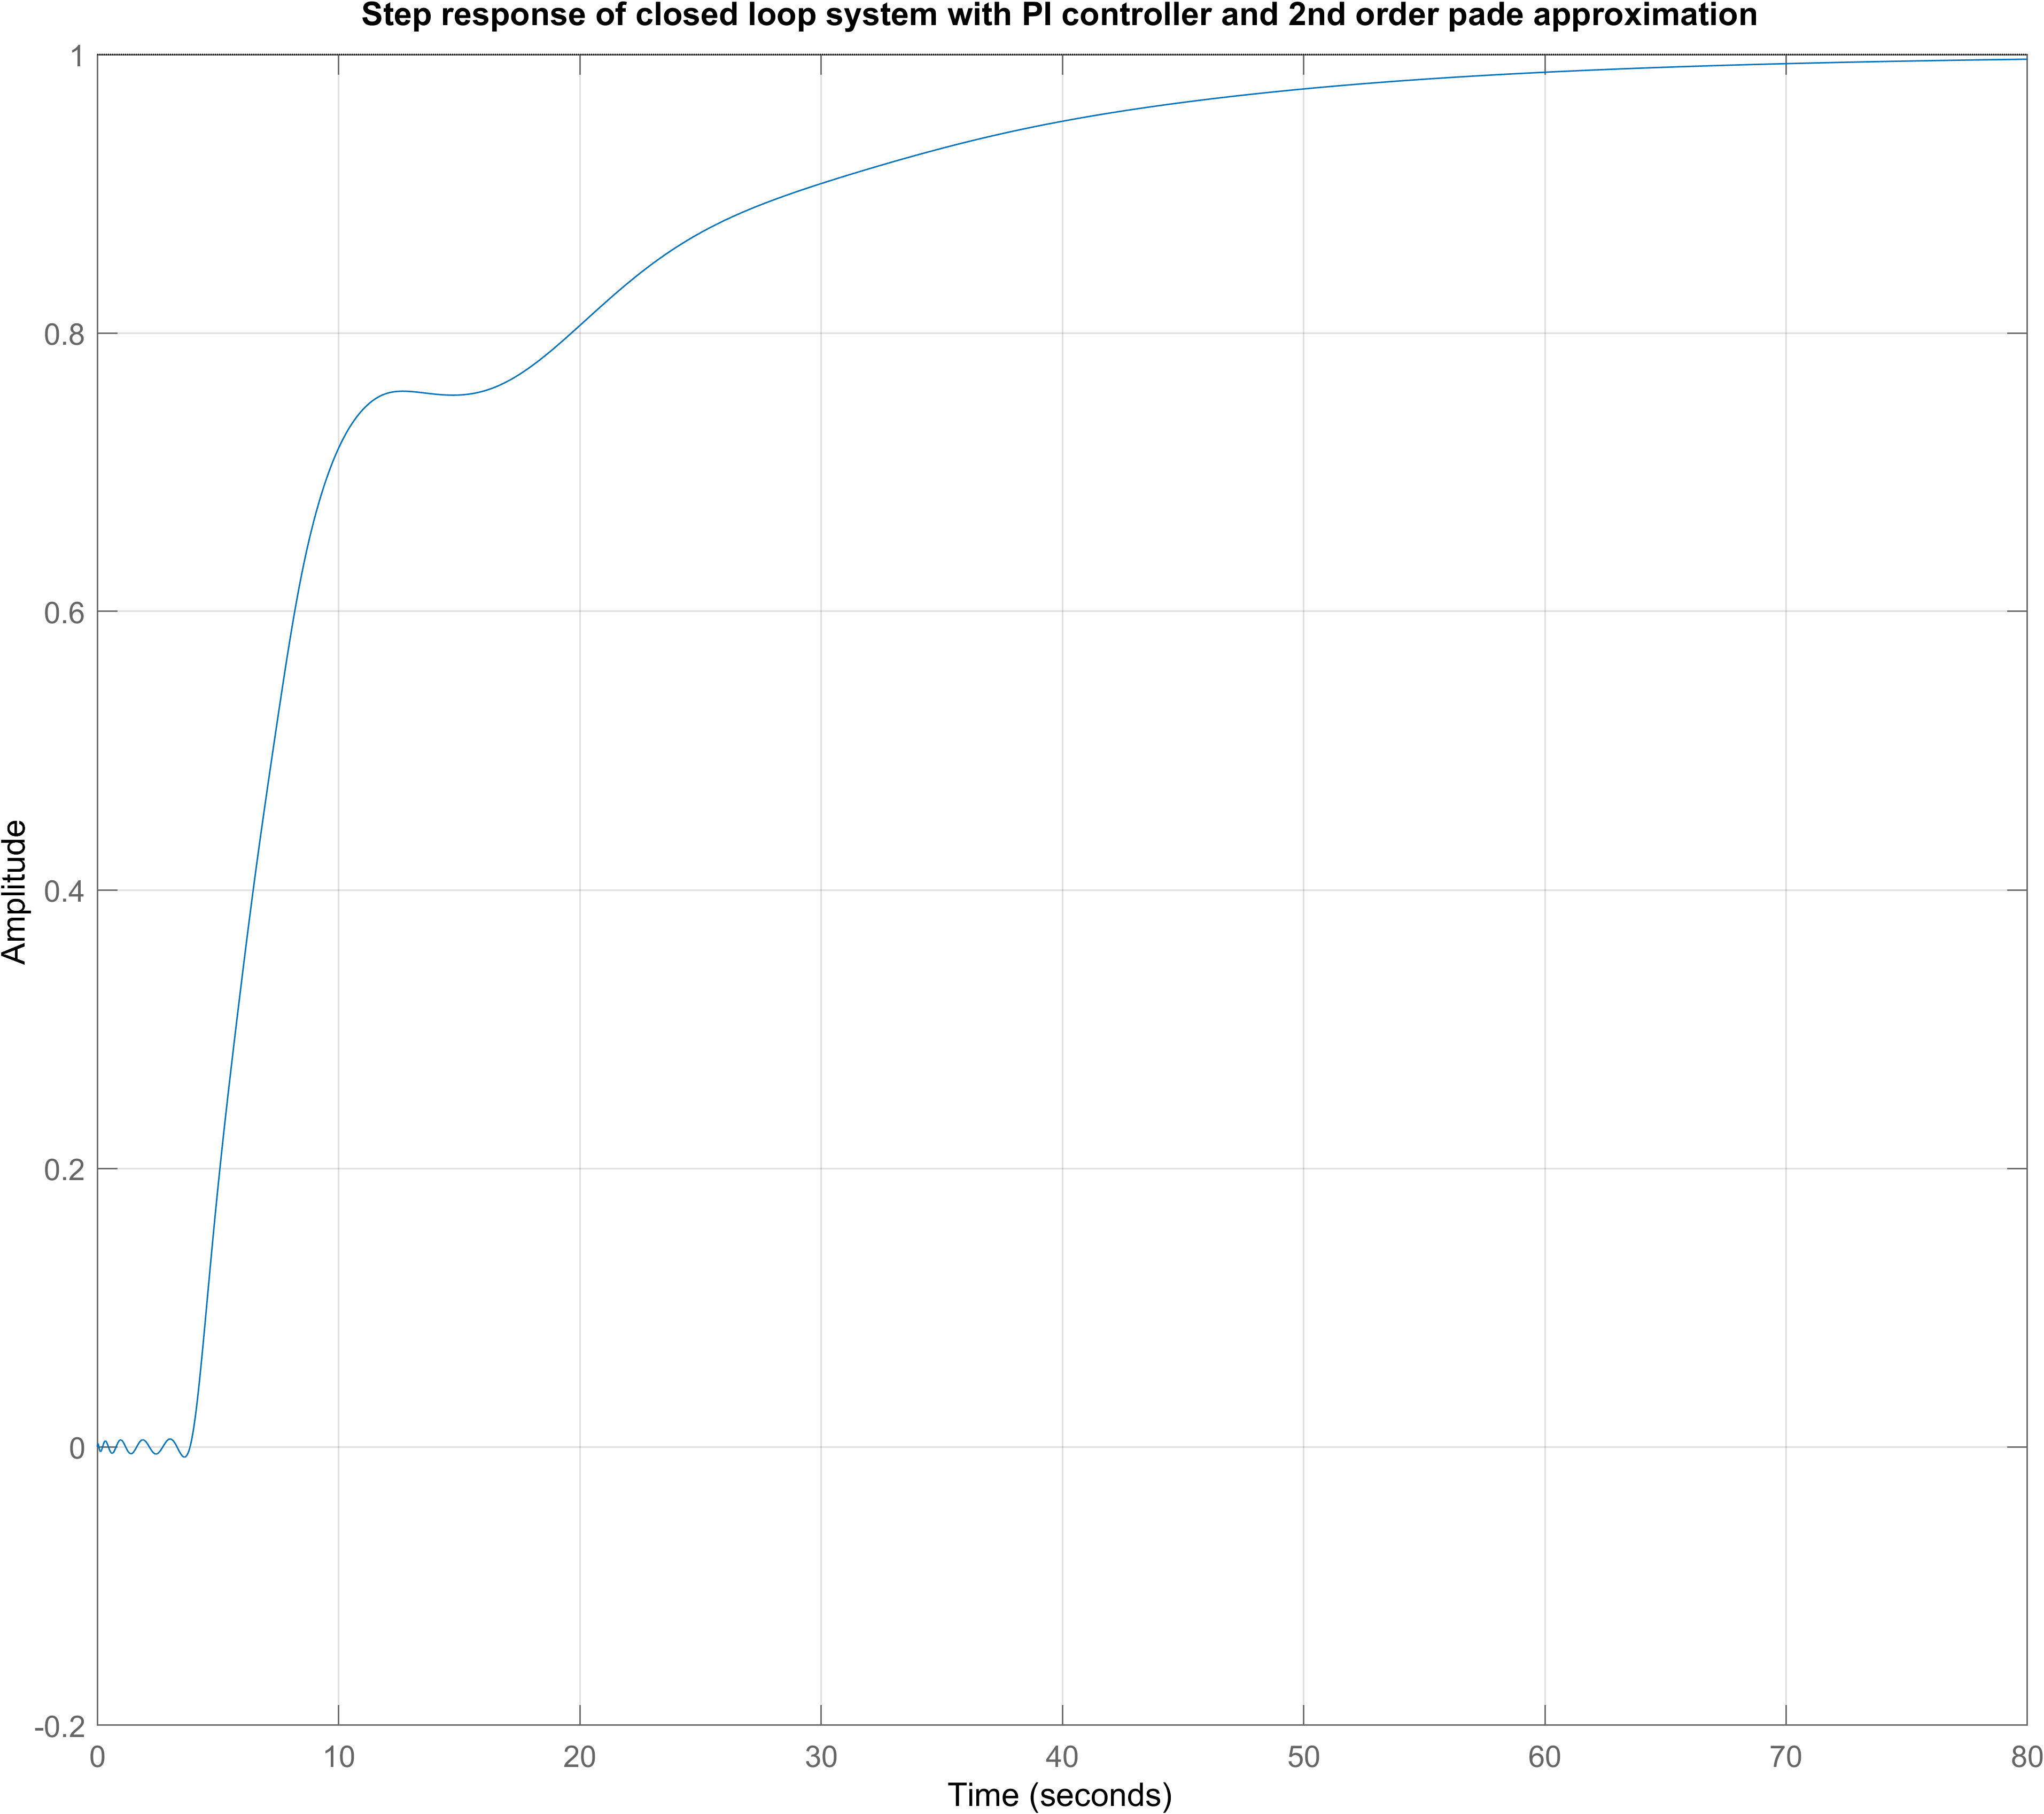
\includegraphics[width=0.8\textwidth]{Pictures/StepResponse_Pade10.png}
	
	\caption{Step response of the closed loop system with a 10th order pade approximation}
	\label{fig:StepResponse_Pade10}
\end{figure}


